\documentclass[11pt]{article}
\usepackage{udec-pset}
\doc{5}{Condensadores y Capacitancia}
\mostrarSoluciones

\usetikzlibrary{arrows.meta, calc, positioning}

% Definición de colores basados en las imágenes
\definecolor{grisAnillo}{RGB}{180,180,180}
\definecolor{placaAzul}{RGB}{175,200,235}
\definecolor{dielClaro}{RGB}{205,225,245}
\definecolor{dielMedio}{RGB}{180,195,210}
\definecolor{dielOscuro}{RGB}{160,180,200}

\begin{document}
\crearEncabezado

\subsection*{Capacitancia y Condensadores}

\begin{boxTeoria}{Definición de Capacitancia}
    Un \textbf{condensador} (o capacitor) es un dispositivo formado por dos conductores separados por un aislante (vacío o dieléctrico) capaz de almacenar carga y energía eléctrica.

    La \textbf{capacitancia} ($C$) es la razón entre la magnitud de la carga $Q$ en cualquiera de los conductores y la magnitud de la diferencia de potencial $\Delta V$ entre ellos:
    \begin{equation*}
        C = \frac{Q}{|\Delta V|} \quad [\unit{\F}] \text{ (Faradios)}
    \end{equation*}
    La capacitancia depende \textbf{exclusivamente de la geometría} de los conductores (área, separación, forma) y del material entre ellos, no de la carga ni del voltaje.
\end{boxTeoria}

\begin{boxTeoria}{Algoritmo General para Calcular Capacitancia}
    Para encontrar teóricamente la capacitancia de cualquier arreglo geométrico, se debe seguir un procedimiento estricto de 4 pasos:
    \begin{enumerate}
        \item \textbf{Asumir carga:} Suponer que los conductores tienen cargas $+Q$ y $-Q$.
        \item \textbf{Calcular $\vv{E}$:} Usar la Ley de Gauss ($\oint \vv{E} \cdot d\vv{A} = \frac{Q_{int}}{\epsilon_0}$) para hallar el campo eléctrico entre los conductores.
        \item \textbf{Calcular $\Delta V$:} Integrar el campo eléctrico desde el conductor negativo al positivo: $\Delta V = -\int_{-}^{+} \vv{E} \cdot d\vv{l}$.
        \item \textbf{Aplicar definición:} Reemplazar en $C = Q/|\Delta V|$. La carga $Q$ se cancelará.
    \end{enumerate}
\end{boxTeoria}

\subsection*{Dieléctricos y Campos en la Materia}

\begin{boxTeoria}{Efecto de un Dieléctrico}
    Un \textbf{dieléctrico} es un material no conductor. Si se inserta un dieléctrico que llena por completo el espacio entre las placas de un condensador, la capacitancia original $C_0$ aumenta por un factor $\kappa$ (o $\epsilon_r$), llamado \textbf{constante dieléctrica} o permitividad relativa:
    \begin{equation*}
        C = \kappa C_0
    \end{equation*}
    Si el condensador está \textbf{aislado} (carga constante), el dieléctrico reduce el campo eléctrico interno y el voltaje ($V = V_0/\kappa$). Si está \textbf{conectado a una batería} (voltaje constante), el dieléctrico permite almacenar más carga ($Q = \kappa Q_0$).
\end{boxTeoria}

\begin{boxTeoria}{Vector Desplazamiento ($\vv{D}$) y Polarización ($\vv{P}$)}
    Al aplicar un campo externo $\vv{E}_0$, las moléculas del dieléctrico se orientan creando un \textbf{Vector Polarización} $\vv{P}$ y acumulando \textbf{cargas ligadas} ($\sigma_p$) en las superficies.

    Para evitar contabilizar estas cargas microscópicas, usamos el \textbf{Vector Desplazamiento Eléctrico} $\vv{D}$, que depende solo de la carga libre (la que controlamos):
    \begin{equation*}
        \vv{D} = \epsilon_0 \vv{E} + \vv{P} = \epsilon \vv{E} \quad \implies \quad \oint \vv{D} \cdot d\vv{A} = Q_{libre}
    \end{equation*}
    Donde $\epsilon = \kappa \epsilon_0$ es la permitividad absoluta del material.
\end{boxTeoria}

\subsection*{Energía y Asociaciones}

\begin{boxTeoria}{Energía Eléctrica Almacenada}
    El trabajo necesario para cargar un condensador se almacena como energía potencial eléctrica en el campo eléctrico creado.
    \begin{equation*}
        U = \frac{1}{2} C (\Delta V)^2 = \frac{Q^2}{2C} = \frac{1}{2} Q \Delta V \quad [\unit{\J}]
    \end{equation*}
    La \textbf{densidad de energía} (energía por unidad de volumen) en el campo eléctrico es $u = \frac{1}{2} \epsilon |\vv{E}|^2$.
\end{boxTeoria}

\begin{boxNota}{Asociación de Condensadores}
    \begin{itemize}
        \item \textbf{Serie:} Misma carga $Q$. El voltaje se divide. $\frac{1}{C_{eq}} = \sum \frac{1}{C_i}$
        \item \textbf{Paralelo:} Mismo voltaje $\Delta V$. La carga se divide. $C_{eq} = \sum C_i$
    \end{itemize}
\end{boxNota}

% EN ARTICLE (La forma correcta)
\noindent
\begin{minipage}[t]{0.6\textwidth}
    \problema Un capacitor está conformado por dos cascarones esféricos conductores concéntricos. Si el cascarón interno tiene un radio $a$, y el cascarón externo un radio $b$. ¿Cuál es la capacitancia de este arreglo?
\end{minipage}% <--- Este porcentaje es vital (evita un espacio invisible)
\hfill
\begin{minipage}[t]{0.4\textwidth}
    \begin{figure}[H]
        \centering
        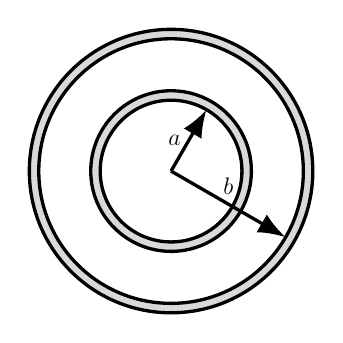
\begin{tikzpicture}[scale=0.6, transform shape]
            % Definición de color por si acaso (ajusta si ya lo tienes definido)
            \colorlet{grisAnillo}{gray!30}

            % Anillo exterior (Más delgado: radios de 2.8 a 3.0)
            \filldraw[fill=grisAnillo, draw=black, very thick, even odd rule]
            (0,0) circle (3.0) (0,0) circle (2.8);

            % Anillo interior (Más delgado: radios de 1.5 a 1.7)
            \filldraw[fill=grisAnillo, draw=black, very thick, even odd rule]
            (0,0) circle (1.7) (0,0) circle (1.5);

            % Flechas y etiquetas actualizadas a las nuevas dimensiones
            % Radio 'a' apunta al borde del anillo interior (1.5)
            \draw[-{Latex[length=3.5mm]}, very thick] (0,0) -- (60:1.5)
            node[midway, left=1pt] {\Large $a$};

            % Radio 'b' apunta al inicio del anillo exterior (2.8)
            \draw[-{Latex[length=3.5mm]}, very thick] (0,0) -- (-30:2.8)
            node[midway, above=2pt] {\Large $b$};
        \end{tikzpicture}
    \end{figure}
\end{minipage}

\begin{solucion}
    Para calcular la capacitancia desde los principios del electromagnetismo, aplicamos el algoritmo de 4 pasos:

    1. \textbf{Asumir carga:} Suponemos una carga $+Q$ en el cascarón interno (radio $a$) y $-Q$  en el cascarón externo (radio $b$) (la esfera encierra completamente a la esfera interna).

    2. \textbf{Campo eléctrico (Ley de Gauss):} Tomamos una superficie gaussiana esférica de radio $r$ tal que $a < r < b$.
    $$\oint \vv{E} \cdot d\vv{A} = \frac{Q_{int}}{\epsilon_0} \implies E(4\pi r^2) = \frac{Q}{\epsilon_0} \implies \vv{E} = \frac{Q}{4\pi\epsilon_0 r^2} \hat{r}$$

    3. \textbf{Diferencia de potencial:} Integramos el campo eléctrico desde el conductor exterior al interior para obtener la diferencia de potencial positiva.
    $$\Delta V = -\int_{b}^{a} \vv{E} \cdot d\vv{r} = -\int_{b}^{a} \frac{Q}{4\pi\epsilon_0 r^2} dr = \frac{Q}{4\pi\epsilon_0} \left( \frac{1}{a} - \frac{1}{b} \right) = \frac{Q(b-a)}{4\pi\epsilon_0 ab}$$

    4. \textbf{Capacitancia:} Aplicamos la definición general $C = Q / \Delta V$.
    $$C = \frac{Q}{\frac{Q(b-a)}{4\pi\epsilon_0 ab}} = \frac{4\pi\epsilon_0 ab}{b - a}$$
\end{solucion}


\noindent
\begin{minipage}[t]{0.6\textwidth}
    \problema Un condensador plano, cuyas armaduras tienen un área de $A [m^2]$ y están separadas por una distancia de $d [m]$, contiene una plancha de material dieléctrico de espesor $d/2 [m]$ y permitividad relativa $\epsilon_r$. Si la diferencia de potencial entre las armaduras es $\Delta V [V]$, Encuentre:
    \begin{enumerate}[label=\alph*)]
        \item La intensidad de campo eléctrico en la región vacía entre las armaduras.
        \item La intensidad de campo eléctrico en el dieléctrico.
    \end{enumerate}
\end{minipage}%
\hfill
\begin{minipage}[t]{0.4\textwidth}

    \begin{figure}[H]

        \centering
        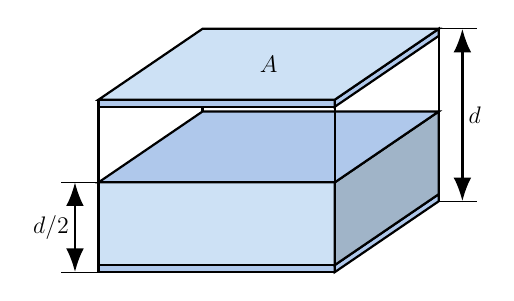
\begin{tikzpicture}[scale=0.6, transform shape]
            % Parámetros de geometría 3D simulada
            \def\w{5}     % Ancho
            \def\h{3.5}   % Altura total entre placas
            \def\dh{1.75} % Altura del dieléctrico (d/2)
            \def\dx{2.2}  % Profundidad en X
            \def\dy{1.5}  % Profundidad en Y
            \def\pt{0.15} % Grosor de la placa

            % 1. PLACA INFERIOR
            \filldraw[fill=placaAzul, draw=black, thick]
            (0,0) rectangle (\w, \pt);
            \filldraw[fill=placaAzul, draw=black, thick]
            (\w,0) -- (\w+\dx, \dy) -- (\w+\dx, \dy+\pt) -- (\w, \pt) -- cycle;

            % 2. DIELÉCTRICO (Mitad inferior)
            % Cara frontal
            \filldraw[fill=dielClaro, draw=black, thick]
            (0,\pt) rectangle (\w, \pt+\dh);
            % Cara lateral derecha
            \filldraw[fill=dielOscuro, draw=black, thick]
            (\w,\pt) -- (\w+\dx, \dy+\pt) -- (\w+\dx, \dy+\pt+\dh) -- (\w, \pt+\dh) -- cycle;
            % Cara superior
            \filldraw[fill=placaAzul, draw=black, thick]
            (0,\pt+\dh) -- (\w, \pt+\dh) -- (\w+\dx, \dy+\pt+\dh) -- (\dx, \dy+\pt+\dh) -- cycle;

            % 3. LÍNEAS DEL ESPACIO DE AIRE (Transparencia)
            \draw[thick] (0, \pt+\dh) -- (0, \h);
            \draw[thick] (\w, \pt+\dh) -- (\w, \h);
            \draw[thick] (\w+\dx, \dy+\pt+\dh) -- (\w+\dx, \dy+\h);
            \draw[thick] (\dx, \dy+\pt+\dh) -- (\dx, \dy+\h);

            % 4. PLACA SUPERIOR
            % Borde frontal
            \filldraw[fill=placaAzul, draw=black, thick]
            (0,\h) rectangle (\w, \h+\pt);
            % Borde lateral
            \filldraw[fill=placaAzul, draw=black, thick]
            (\w,\h) -- (\w+\dx, \dy+\h) -- (\w+\dx, \dy+\h+\pt) -- (\w, \h+\pt) -- cycle;
            % Cara superior
            \filldraw[fill=dielClaro, draw=black, thick]
            (0,\h+\pt) -- (\w, \h+\pt) -- (\w+\dx, \dy+\h+\pt) -- (\dx, \dy+\h+\pt) -- cycle;

            % 5. ETIQUETAS Y COTAS
            % Área A
            \node at (\w/2 + \dx/2, \h+\pt + \dy/2) {\Large $A$};

            % Cota d/2 (Izquierda)
            \draw (0, 0) -- (-0.8, 0);
            \draw (0, \pt+\dh) -- (-0.8, \pt+\dh);
            \draw[{Latex[length=3mm]}-{Latex[length=3mm]}, thick]
            (-0.5, 0) -- (-0.5, \pt+\dh) node[midway, left] {\Large $d/2$};

            % Cota d (Derecha)
            \draw (\w+\dx, \dy) -- (\w+\dx+0.8, \dy);
            \draw (\w+\dx, \dy+\h+\pt) -- (\w+\dx+0.8, \dy+\h+\pt);
            \draw[{Latex[length=3mm]}-{Latex[length=3mm]}, thick]
            (\w+\dx+0.5, \dy) -- (\w+\dx+0.5, \dy+\h+\pt) node[midway, right] {\Large $d$};
        \end{tikzpicture}
    \end{figure}
\end{minipage}

\noindent
\begin{minipage}[t]{0.6\textwidth}
    \problema Un condensador de placas paralelas tiene capacidad $C_0$ cuando el dieléctrico entre sus placas es vacío. Si tres bloques, cada uno con un área equivalente a la mitad del área de las placas, se insertan entre las placas, tal como se muestra en la figura. ¿Cuál es la capacidad de este dispositivo?  (Considerando las permitividades relativas $\kappa_1$, $\kappa_2$ y $\kappa_3$).
\end{minipage}%
\hfill
\begin{minipage}[t]{0.4\textwidth}
    \begin{figure}[H]
        \centering
        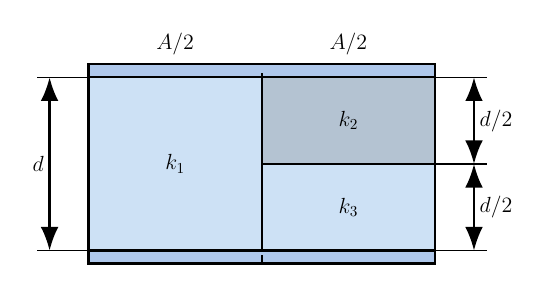
\begin{tikzpicture}[scale=0.55, transform shape]
            % PLACAS
            % Placa inferior
            \filldraw[fill=placaAzul, draw=black, thick] (0,-0.3) rectangle (8,0);
            % Placa superior
            \filldraw[fill=placaAzul, draw=black, thick] (0,4) rectangle (8,4.3);

            % DIELÉCTRICOS
            % k1 (Izquierda)
            \filldraw[fill=dielClaro, draw=black, thick] (0,0) rectangle (4,4);
            \node at (2,2) {\Large $k_1$};

            % k2 (Derecha Superior)
            \filldraw[fill=dielMedio, draw=black, thick] (4,2) rectangle (8,4);
            \node at (6,3) {\Large $k_2$};

            % k3 (Derecha Inferior)
            \filldraw[fill=dielClaro, draw=black, thick] (4,0) rectangle (8,2);
            \node at (6,1) {\Large $k_3$};

            % Línea divisoria central
            \draw[dashed, thick] (4,-0.3) -- (4,4.3);

            % ETIQUETAS Y COTAS
            % Áreas
            \node[above] at (2, 4.4) {\Large $A/2$};
            \node[above] at (6, 4.4) {\Large $A/2$};

            % Cota d (Izquierda)
            \draw (0,0) -- (-1.2,0);
            \draw (0,4) -- (-1.2,4);
            \draw[{Latex[length=3mm]}-{Latex[length=3mm]}, thick]
            (-0.9,0) -- (-0.9,4) node[midway, left] {\Large $d$};

            % Cotas d/2 (Derecha)
            \draw (8,0) -- (9.2,0);
            \draw (8,2) -- (9.2,2);
            \draw (8,4) -- (9.2,4);

            \draw[{Latex[length=3mm]}-{Latex[length=3mm]}, thick]
            (8.9,0) -- (8.9,2) node[midway, right] {\Large $d/2$};
            \draw[{Latex[length=3mm]}-{Latex[length=3mm]}, thick]
            (8.9,2) -- (8.9,4) node[midway, right] {\Large $d/2$};
        \end{tikzpicture}
    \end{figure}
\end{minipage}

\end{document}